\chapter{Machine Learning for static data: state of the art}
\label{chap:premierchapitre}
\minitoc

%\noindent Introduction du chapitre:
%\begin{itemize}
%	\item Hypothèse: considérer les séries temporelles comme des vecteurs de données statiques
%	\item Appliquer les méthodes classiques de Machine Learning
%	\item NB : Faire bien attention à bien utiliser MES notations
%\end{itemize}


\fbox{  \parbox{0.9\textwidth}{
In this chapter, we first present what a time series is. Then, we consider time series as static data by vectorizing them to apply machine learning algorithms used for classification and regression. We detail some of these learning algorithms. Finally, we review the protocol used to learn the best fitting of the hyper-parameters of these algorithms and how we evaluate and compare the different algorithms performances.
% Time series and more generally temporal data are data objects that are frequently common nowadays. By considering time series as a vector, one can use classic learning algorithms that are designed for static data. We first present a state of the art of some learning algorithms used for classification and regression. Then, we review the protocol used to learn the best fitting of the hyper-parameters of these algorithms and how we evaluate and compare the different algorithms performances.
}  }

\section{Definition of a time series}
Let $\textbf{x}_i=(x_{i1}, x_{i2}, ..., x_{iT})$ be a univariate time series of length $T$. We call time series, a collection of numerical observations made sequentially in the time. It is characterized by a finite number of realized observations made at discrete instants of time $t=1,...,T$. Moreover, each observation $x_{it}$ is bounded (i.e. the infinity is not a valid value: $x_{it} \neq \pm \infty$). The time series $\textbf{x}_i$ is said to be univariate if the collection of observations $x_{it}$ comes from the observations of one variable (i.e. it has been measured by one sensor, the temperature for example). When the observations are made from $Q$ variables (several sensors such as the temperature, the pressure, etc.), the time series is said multivariate and is denoted $\textbf{x}_i=(\textbf{x}_{i,1}, ...., \textbf{x}_{i,Q})=(x_{i1,1}, ..., x_{iT,1},x_{i1,2}, ..., x_{iT,2}, ..., x_{i1,Q}, ..., x_{iT,Q})$. We consider in the following for simplification purpose univariate time series. 

Fig.~\ref{fig:time_series_example} illustrates a model for time series proposed by Chatfield in [\cite{Chatfield2004a}]. It states that a time series can be decomposed into 3 components: a trend, a cycle (periodic component) and a residual (irregular variations). 

\begin{figure}[h!]
\centering
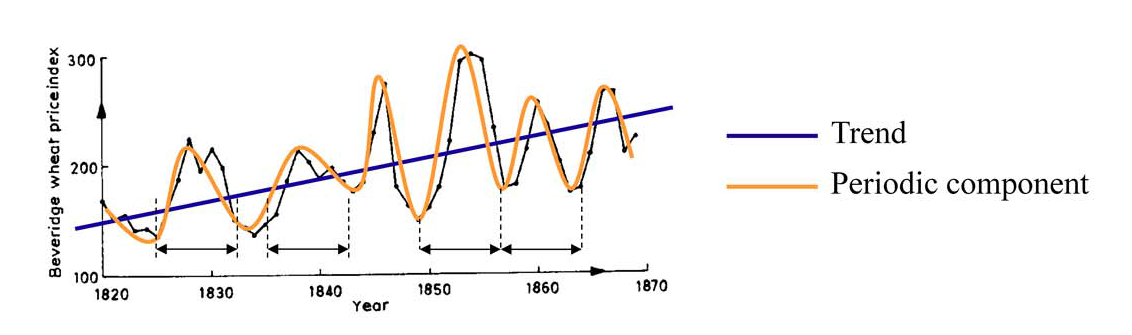
\includegraphics[width=1\linewidth]{images/time_series_example}
\caption{The Beveridge wheat price index is the average in nearly 50 places in various countries measured in successive years from 1500 to 1869. \protect\footnotemark}
\label{fig:time_series_example}
\end{figure}
\footnotetext{This time series can be downloaded from \url{http://www.york.ac.uk/depts/maths/data/ts/ts04.dat}}

\noindent According to Chatfield, most time series exhibit a variation at a fixed period of time (seasonality) such as for example the seasonal variation of temperature. Beyond this cycle, there exist either or both a long term change in the mean (trend) that can be linear, quadratic, and a periodic (cyclic) component. By definition, a signal is periodic of period $R$ if $x_{t+R}=x_t$ for all time instants $t$. In practice, this condition is not valid for real time series.

Time series can be found in various emerging applications such as sensor networks, smart buildings, social media networks or Internet of Things (IoT) [\cite{Najmeddine2012,Nguyen2012,Yin2008}]. They are involved in classification, regression and clustering problems. Due to their temporal and structured nature, time series constitute complex data to be analyzed by classic machine learning approaches. One common technics consists in considering time series as a static vector data and then to use classic machine learning algorithms.


% Nous désignons par données temporelles des données numériques évoluant dans le temps, dites communément séries temporelles, ou des suites chronologiques de données symboliques dites séquences temporelles. Plus généralement, on désigne par données de séquences toute collection de données ordonnées selon un critère qui peut être sémantique, biologique, temporel ou autre ; c’est le cas, par exemple, des séquences de mots dans un texte ; on parle alors d’ordre syntaxique, de séquences d’acides aminés composant une chaîne d’ADN ou de peptides constituant une protéine.


%----------------------------------------------------------------------------
\section{Machine learning algorithms}

We are going to detail now a few number of machine learning algorithms used classically to solve classification or regression problems ($k$-Nearest Neighbors ($k$-NN) and Support Vector Machine (SVM)). Other algorithms are popular nowadays (Deep neural network, Decision tree, Relevance vector machine, etc.) but we will focus on $k$-NN and SVM because these learning algorithms are based on the comparison of objects (time series in our case) through a distance measure, notion that we will develop in the next chapter and that will be at the base of our proposition.

\subsection{Classification, regression and clustering}
Let $\textbf{X}=\{\textbf{x}_i,y_i\}_{i=1}^n$ be a set of $n$ time series $\textbf{x}_i$ and $y_i$ their corresponding labels. The aim of Machine learning is to learn a relation (model) $f$ between the time series $\textbf{x}_i$ and their labels $y_i$ based on examples. This relationship can include static relationships, correlations, dynamic relationship, etc. [\cite{Dreyfus2006}]. 

The idea of Machine learning (also refer as Pattern learning or Pattern recognition) is to imitate with algorithms executed on computers, the ability of living beings to learn from examples. For example, to teach a child how to read letters, we show him during the learning phase labeled examples of letters ('A', 'B', 'C', etc.) written in different styles and fonts. We don't give him a complete and analytic description of the topology of the characters but labeled examples. After the learning phase (testing phase), we want the child to be able to recognize and to label correctly the letters that have been seen during the training, and also to generalize to new instances. In the same spirit, after the training phase based on labeled examples, the model $f$ has to be able to generalize on the testing phase, i.e. to give a correct prediction for new instances that haven't been seen during the training.

When $y_i$ are class labels (i.e. class 'A', 'B', 'C'), learning the model $f$ is a classification problem; when $y_i$ is a continuous value (i.e. the energy consumption in a building), learning $f$ is a regression problem. Both problems corresponds to supervised learning as $\textbf{x}_i$ and $y_i$ are known during the training phase \textcolor{red}{[biblio]}. When a part of the labels $y_i$ are known and an other part of $y_i$ is unknown during training, learning $f$ is a semi-supervised problem \textcolor{red}{[biblio]}. Finally, when the labels $y_i$ are unknown, learning $f$ refers to a clustering problem (unsupervised learning) \textcolor{red}{[biblio]}. Our work will focus on supervised learning (classification, regression).


\subsection{$k$-Nearest Neighbors ($k$-NN)}
\begin{itemize}
	\item Donner l'intuition
	\item Formaliser le problème en tant que problème d'optimisation
	\item Présenter les extensions (kNN pondéré), extension à la régression
	\item Soulever le fait que la résolution du problème fait intervenir une notion de distance entre les individus (time series)	
	\item Donner les arguments qui permettent de dire pourquoi utiliser un 1-NN permet de faire une évaluation de métriques (Ding)
\end{itemize}

A simple approach to classify objects is to consider that "close" objects have a great probability to belong to the same class. Given a test sample (in our case, a time series) $\textbf{x}_i$, one can decide that this object belong to the same class of its nearest neighbor in the training set. More generally, we can consider the $k$ nearest neighbors of an unknown object $\textbf{x}_i$, and we assign its label $y_i$ to the majority class of its $k$ nearest neighbors (vote). This algorithm is refer as the $k$ nearest neighbors algorithm ($k$-NN) [\cite{Dreyfus2006}].

\begin{figure}
\centering
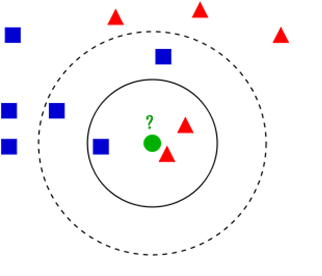
\includegraphics[width=0.4\linewidth]{images/kNN_example}
\caption{Example of $k$-NN classification. The test sample (green circle) is classified either to the first class (blue squares) or to the second class (red triangles). If $k = 3$ (solid line circle) it is assigned to the second class because there are 2 triangles and only 1 square inside the inner circle. If $k = 5$ (dashed line circle) it is assigned to the first class (3 squares vs. 2 triangles inside the outer circle).}
\label{fig:kNN_example}
\end{figure}

\noindent The key point in the $k$-NN algorithm is that the notion of "closeness" between objects is based on the computation of a distance measure. Let $D$ be a distance measure. Usally, for static data, standard metrics are the Euclidean Distance, the Minkowski Distance or the Mahalanobis Distance. Solving the 1-NN classification problem is equivalent to solve the optimization problem: \\
\noindent For a new instance $\textbf{x}_j$, $\forall i \in \{1...n\}$,
\begin{equation}
y_j = y_{i}
\end{equation}
where $i={\underset{i \in \{1...n\},}{argmin}  D(\textbf{x}_i,\textbf{x}_j)}$.

The $k$-NN algorithm can be extended to estimate continous labels (regression problems). The procedure is similar. The label $y_j$ is defined as :
\begin{equation}
y_j = \sum_{i=1}^{k} y_{i}
\end{equation}
where $i$ corresponds to the index of the $k$-nearest neighbors. \textbf{[biblio]}

Variant kNN (kNN weighed, fuzzy kNN)

Pros of the kNN
% \textcolor{red}{Accuracy evaluation answers one of the most important questions about a similarity measure: why is this a good measure for describing the (dis)similarity between time series? Surprisingly, we found that accuracy evaluation is usually insufficient in existing literature: it has been either based on subjective evaluation, e.g., [4, 9], or using clustering with small data sets which are not statistically significant, e.g., [31, 40]. In this work, we use an objective evaluation method recently proposed [25]. The idea is to use a one nearest neighbor (1NN) classifier [17, 32] on la- belled data to evaluate the efficacy of the distance measure used. Specifically, each time series has a correct class label, and the classifier tries to predict the label as that of its nearest neighbor in the training set. There are several advantages with this approach. First, it is well known that the underlying distance metric is critical to the performance of 1NN classifier [32], hence, the accuracy of the 1NN classifier directly reflects the effectiveness of the similarity measure. Second, the 1NN classifier is straightforward to implement and is parameter free, which makes it easy for anyone to reproduce our results. Third, it has been proved that the error ratio of 1NN classifier is at most twice the Bayes error ratio [36]. Finally, we note that while there have been attempts to classify time series with decision trees, neural networks, Bayesian networks, supporting vector machines etc., the best published results (by a large margin) come from simple nearest neighbor methods [42]}


Cons of the kNN
%Curse of Dimensionality
%* Distance usually relates to all the attributes and assumes all
%of them have the same effects on distance
%* The similarity metrics do not consider the relation of
%attributes which result in inaccurate distance and then impact
%on classification precision. Wrong classification due to
%presence of many irrelevant irrelevant attributes attributes is often termed as the
%curse of dimensionality
%* For example: Each instance is described by 20 attributes out
%of which only 2 are relevant in determining the classification
%of the target function. In this case, instances that have
%identical values for the 2 relevant attributes may
%nevertheless be distant from one another in the 20
%dimensional instance space
%(http://www.csee.umbc.edu/~tinoosh/cmpe650/slides/K_Nearest_Neighbor_Algorithm.pdf)


DUDA
The computational complexity of the nearest-neighbor algorithm - both in space (storage of prototypes) and time (search) - has received a great deal of analysis. Suppose we have n labelled training samples in d dimensions, and seek to find the closest to a test point x (k = 1). In the most naive approach we inspect each stored point in turn, calculate its Euclidean distance to x, retaining the identity only of the current closest one. Each distance calculation is O(d), and thus this search is 0(dn2). An alternative but straightforward parallel implementation is shown in Fig. 4.17, which is 0(1) in time and O(n) in space.


\subsection{Support Vector Machine (SVM)}
\begin{itemize}
	\item Présenter le principe général des SVM en commençant par l'intuition.
	\item Forme primale: donner la formulation primale du problème d'optimisation
	\item Forme duale: montrer commencer passer de la forme primal à la forme dual.
	\item A partir de la forme duale, passer au kernel
	\item Finir par la complexité du SVM en apprentissage ($o(N^3p)$) et en test (limités aux nombres de support vectors) et les interprétations des supports vectors.
	\item Expliquer la modification du problème initiale avec une régularisation L1 sur le terme de régularisation et nous permet d'avoir une solution sparse (donner 1 cas où la solution sparse est meilleur).
	\item Expliquer que dans le cadre de données non-balancées, il faut ajouter des termes pour rebalancer l'équation du SVM
\end{itemize}
\subsection{Other classification algorithms}
\begin{itemize}
	\item S'intéresser au Deep neural network (à la mode en ce moment)
	\item RVM, Decision Tree, 
	\item Ne pas trop développer
	\item Dans notre cas, on ne s'intéressera pas à ce type d'algorithmes (type deep learning) car il ne repose pas sur une notion de distance et les features qui sont trouvés ne sont pas interprétables
\end{itemize}
%----------------------------------------------------------------------------
\section{Learning protocol}
\subsection{Learning framework}
\begin{itemize}
	\item Learning framework (train, validation, test): la plupart des algorithmes requiert l'optimisation d'un hyper-paramètre. Le jeu de train permet d'apprendre les meilleurs hyper-paramètres.
	\item Cross-validation (pourquoi on fait de la cross-validation, comment on la fait (Faire un schéma))
\end{itemize}	

\subsection{Model evaluation}
\begin{itemize}
	\item Classification Error et test de significativité
	\item Regression Error
\end{itemize}

\subsection{Data pre-processing}
\begin{itemize}
	\item Normalization
	\item PCA
\end{itemize}

%----------------------------------------------------------------------------
\section{Limits of classical technics}
\begin{itemize}
	\item The concept of order of temporal data in not take into account (dynamic, frequence, etc.)
	\item Introduction to next chapter: all of these algorithms (kNN, SVM, etc.) are based on a notion of distance or similarity between objects to compare/classify. Let consider now the object time series and let recall the concept of distance between time series
\end{itemize}

%%% Local Variables: 
%%% mode: latex
%%% TeX-master: "../roque-phdthesis"
%%% End: 
